\chapter{工具}
《Linux多线程服务端编程——使用muduo C++网络库》这本书是我自己用 \LaTeX 排版的,
在排版过程中也积累了一些小工具,本章把它们一一展示出来。
不少工具都直接基于开源的 iText PDF 库,可从 \myurl{http://itextpdf.com/} 下载,
我用的是 \fn{itextpdf-5.3.0.jar}。另外一些则用到了 Ghostscript,
可直接用 \fn{apt-get} 安装。

\subsubsection{下载}

Groovy 版本位于 \myurl{https://github.com/chenshuo/typeset/tree/master/tools}

Java 版本位于 \myurl{https://github.com/chenshuo/recipes/tree/master/java/pdf}

各个工具的输出示例位于 \myurl{http://vdisk.weibo.com/s/kT4fL}

\section{统计中文字数}
\LaTeX 没有像 Word 那样自带中文字数统计功能,加上 \LaTeX 源文件中有许多控制字符,
不能通过文件大小准确获知其中有多少汉字。
为此我用C写了一个统计中文字数的小工具,名为 \fn{cwc},即 chinese word counter,
这个工具可以处理GBK、Unicode (UCS-2)、UTF-8这三种编码的文件。\mpar{补例子}
源码位于 \myurl{https://github.com/chenshuo/recipes/tree/master/utility}。
以下是一次运行的输出。
\begin{Code}
$ cwc chapTools.tex chapRules.tex
   119   1012    5329 chapTools.tex (UTF-8)
    13     33     167 chapRules.tex (UTF-8)
   132   1045    5496 total
  行数   字数   字节数
\end{Code}

\section{PDF内容对比(dif\/f\,)}
在书籍出版之后,每次印刷都可能修订一些内容,
在把新的PDF文件交给出版社的同时,也要通知哪些页码有改动,
方便出版社印刷。
由于PDF是二进制格式,无法直接对比新旧PDF文件,
于是我写了一个 \fn{diffpdf.sh} 小工具用来找出哪些页面的内容有改动。
这个工具的思路很土,就是先用 Ghostscript 把PDF按页渲染为多个PNG文件,
然后用 \fn{diff(1)} 比较新旧两个PDF渲染出来的这些PNG文件是否相同。
然后用 Python 脚本(\fn{diffpng.py})将两个PNG文件的不同之处用红色高亮显示出来。例如:

\vspace{1ex}
\centerline{
\includegraphics{diffpng.png}}

\section{PDF截取}
为了在网上公布样张,我需要从整书中截取一部分页码,
另存为PDF文件,这用 \fn{pdftk} 最方便了。
例如
\begin{Code}
pdftk book.pdf cat 1-16 output preamble.pdf     # 前言和目录
pdftk book.pdf cat 19-46 output chap1.pdf       # 第1章
pdftk book.pdf cat 577-end output appendix.pdf  # 附录
\end{Code}


\section{PDF页码编号}

\LaTeX 的 \fn{hyperref} 宏包可以为生成的PDF设置“逻辑页码”,
例如前言目录用罗马数字,正文用阿拉伯数字。
不过经过 \fn{pdftk} 截取之后就失效了。
为此我编写了 \fn{pagenum.groovy} 工具,用来添加逻辑页码。例如
\begin{Code}
pagenum.groovy '1e,3r' preamble.pdf  # 第1、2页是封面,没有页码;第3页开始用罗马数字
pagenum.groovy '1n3'   chap1.pdf     # 第1章第1页的逻辑页码是3
pagenum.groovy '1n561' appendix.pdf  # 附录第1页的逻辑页码是561
\end{Code}


\section{PDF剪裁(crop)}
为了充分利用屏幕空间,也便于在电子阅读器(iPad、Kindle)上阅读校对书稿,
我一般会把PDF剪裁为版心大小。
例如下面左图是原始PDF,为纸张大小;右图是按固定Crop Box剪裁之后的版心。
\mpar{固定剪裁}

\vspace{1ex}
\centerline{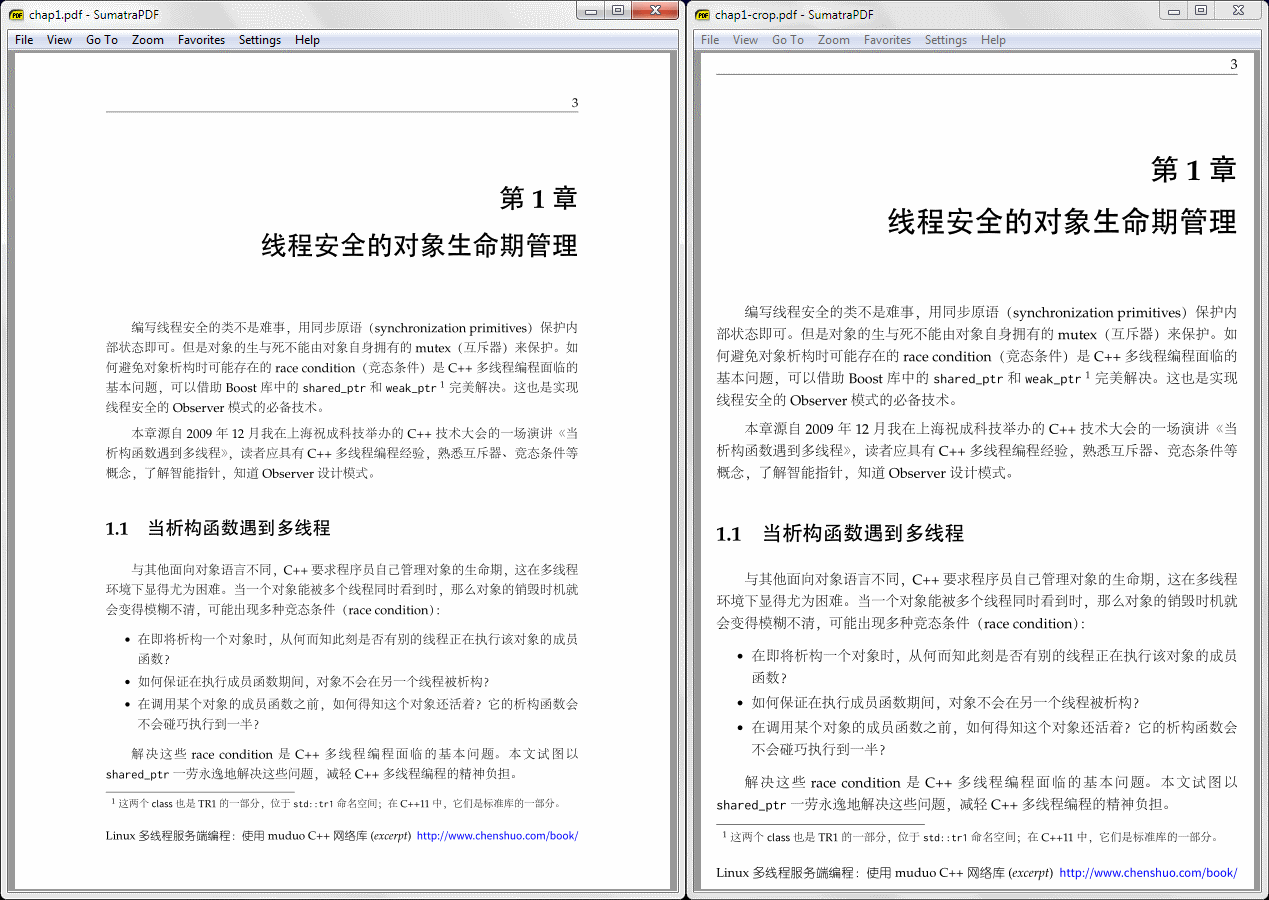
\includegraphics[scale=0.4]{crop.png}}

剪裁工具是 \fn{crop.groovy},设好 \sfn{CLASSPATH} 后可直接在命令行运行。
其核心是根据版心和纸张尺寸算出左下角和右上角左边,然后剪裁每一页。
这个工具不管PDF的内容,如果需要根据页面内容剪裁PDF,\mpar{按内容剪裁}
可以使用Heiko Oberdiek编写的 \fn{pdfcrop} 工具,地址如下:

\begindot
\item \myurl{http://www.ctan.org/tex-archive/support/pdfcrop}
\item \myurl{http://code.google.com/p/pdfcrop2/}
\myenddot

%\subsection


\section{PDF拼接(two-up)}
有时候想在宽屏上同时阅读左右两页的书稿,除了可以用PDF阅读器本身的多页显示功能,
我还常常自己做二合一(two-up)。
这样得到的PDF也可以打印出来看,既节约纸张,而且与原稿是1:1大小。生成的PDF效果如下图。

\vspace{1ex}
\centerline{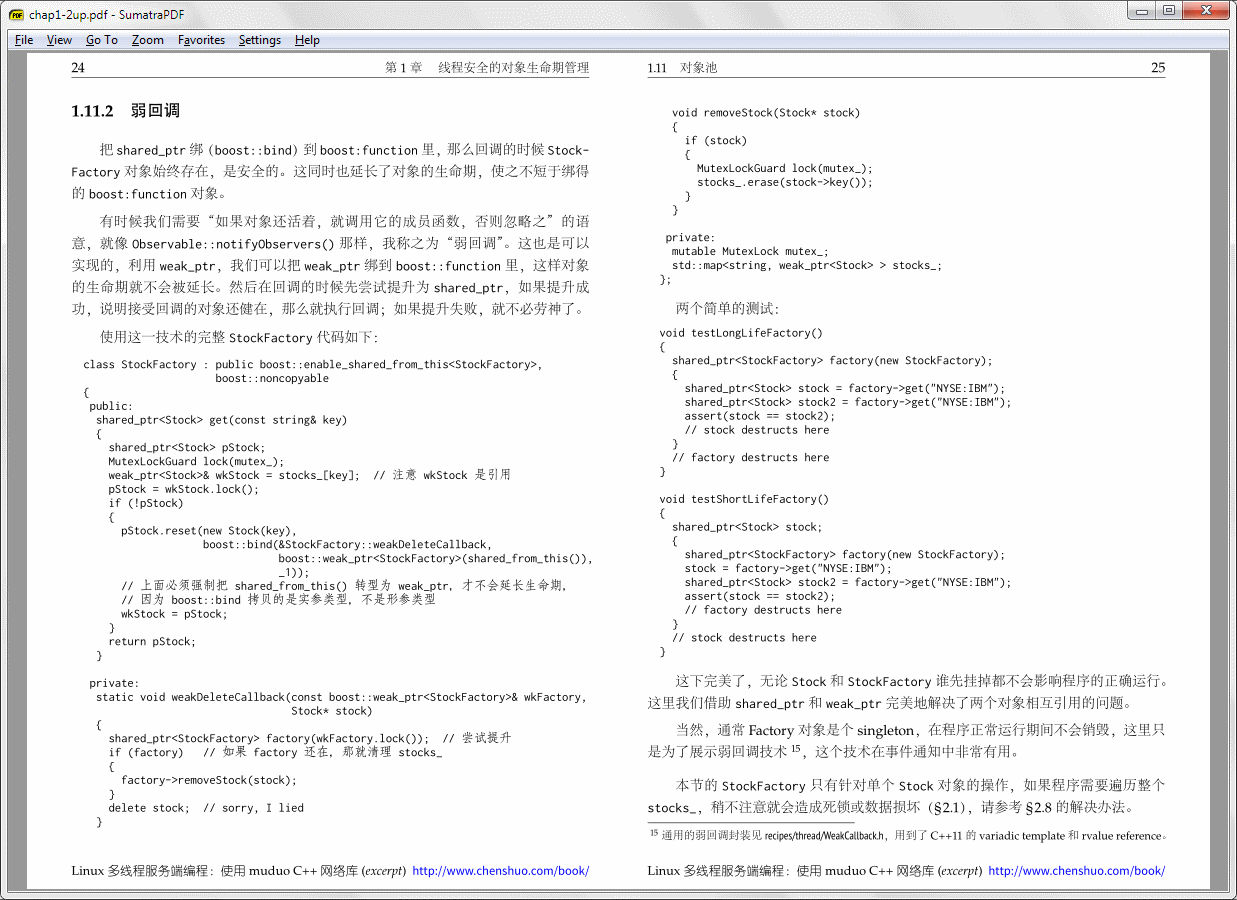
\includegraphics[scale=0.4]{twoup.png}}

二合一工具是 \fn{twoup.groovy},其核心是算出左右两页在合页中的起始坐标。

\section{PDF小册子(booklet)}

有时候我会把一章的内容打印出来,装订成一本小册子,这样读起来有翻书的感觉。
为了节约纸张,在打印之前要拼版,这样一张纸双面能打印4个页码。
例如8页内容可以打印到两张A4纸上:

\vspace{1ex}
\centerline{\includegraphics{booklet-1.eps}\qquad\includegraphics{booklet-2.eps}}

对折、叠好,骑缝订之后就是一本小册子了。

\begin{center}

第一张纸的正反两面打印:

\vspace{1ex}
\includegraphics{booklet-3.eps}\qquad\includegraphics{booklet-4.eps}

\vspace{1em}
第二张纸的正反两面打印:

\vspace{1ex}
\includegraphics{booklet-5.eps}\qquad\includegraphics{booklet-6.eps}
\end{center}

小册子工具是 \fn{booklet.groovy},其核心是算出每面纸应该放哪两个页码的原始内容。

装订这种小册子要用骑缝订,可用旋转订书机
\footnote{\myurl{http://www.amazon.cn/dp/B0080AF0FM} \quad \myurl{http://product.dangdang.com/product.aspx?product_id=1141537002}}。
一本小册子一般应该控制在10页纸左右,即40个页码,再厚就订不透了。

\section{PDF字体嵌入}
出版社拿到作者提供的终稿PDF之后,如果没有进一步修改,就会准备印刷了。
第一步是让出片公司打印出胶片,即“出片”。
这种公司使用的操作系统很可能与作者不同,特别是安装的字体可能不一致。
为了防止出现文字乱码或字体错乱,出片公司一般都会要求提供嵌入全部字体的PDF文件。
